%% Exemplo de utilizacao do estilo de formatacao normas-utf-tex (http://normas-utf-tex.sourceforge.net)
%% dúvidas acessar o site acima
%%
%%
%% Autores: (200?-2011) Hugo Vieira Neto (hvieir@utfpr.edu.br)
%%          (200?-2011) Diogo Rosa Kuiaski (diogo.kuiaski@gmail.com)
%%          (2011-2017) Marcos Talau <talau@users.sourceforge.net>
%% Colaborador:
%%          (2011) César M. Vargas Benitez <cesarvargasb@gmail.com>

%%
%% IMPORTANTE: O texto está escrito com acentuação antiga, atualmente você
%%             pode escrever acentos sem precisar de códigos para tal.
%%

\documentclass[openright]{normas-utf-tex} %openright = o capitulo comeca sempre em paginas impares
%\documentclass[oneside]{normas-utf-tex} %oneside = para dissertacoes com numero de paginas menor que 100 (apenas frente da folha) 

% force A4 paper format
\special{papersize=210mm,297mm}

\usepackage[alf,abnt-emphasize=bf,bibjustif,recuo=0cm, abnt-etal-cite=2, abnt-etal-list=99]{abntcite} %configuracao correta das referencias bibliograficas.

\usepackage[brazil]{babel} % pacote portugues brasileiro
\usepackage[utf8]{inputenc} % pacote para acentuacao direta
\usepackage{amsmath,amsfonts,amssymb} % pacote matematico
\usepackage{graphicx} % pacote grafico
\usepackage{times} % fonte times
\usepackage[final]{pdfpages} % adicao da ata

%Podem utilizar GEOMETRY{...} para realizar pequenos ajustes das margens. Onde, left=esquerda, right=direita, top=superior, bottom=inferior. P.ex.:
%\geometry{left=3.0cm,right=1.5cm,top=4cm,bottom=1cm} 

% ---------- Preambulo ----------
\instituicao{Universidade Tecnológica Federal do Paraná} % nome da instituicao
\programa{Programa de Pós-graduação em Engenharia Elétrica e Informática Industrial} % nome do programa
\area{Informática Industrial} % [Engenharia Biom\'edica] ou [Inform\'atica Industrial] ou [Telem\'atica]

\documento{Dissertação} % [Disserta\c{c}\~ao] ou [Tese]
\nivel{Mestrado} % [Mestrado] ou [Doutorado]
\titulacao{Mestre} % [Mestre] ou [Doutor]

\titulo{{Sistema autonomo de gerenciamento de luzes}} % titulo do trabalho em portugues
\title{\MakeUppercase{Title in English}} % titulo do trabalho em ingles

\autor{Luis Denis Pliskievski de Lara} % autor do trabalho
\cita{LARA, Luis Denis Pliskievski de} % sobrenome (maiusculas), nome do autor do trabalho

\palavraschave{Palavra-chave 1, Palavra-chave 2, ...} % palavras-chave do trabalho
\keywords{Keyword 1, Keyword 2, ...} % palavras-chave do trabalho em ingles

\comentario{\UTFPRdocumentodata\ apresentada ao \UTFPRprogramadata\ da \ABNTinstituicaodata\ como requisito parcial para obtenção do grau de ``\UTFPRtitulacaodata\ em Ciências'' -- Área de Concentração: \UTFPRareadata.}

\orientador{Nome do Orientador} % nome do orientador do trabalho
%\orientador[Orientadora:]{Nome da Orientadora} % <- no caso de orientadora, usar esta sintaxe
%\coorientador{Nome do Co-orientador} % nome do co-orientador do trabalho, caso exista
%\coorientador[Co-orientadora:]{Nome da Co-orientadora} % <- no caso de co-orientadora, usar esta sintaxe
%\coorientador[Co-orientadores:]{Nome do Co-orientador} % no caso de 2 co-orientadores, usar esta sintaxe
%\coorientadorb{Nome do Co-orientador 2}	% este comando inclui o nome do 2o co-orientador

\local{Curitiba} % cidade
\data{\the\year} % ano automatico

% desativa hifenizacao mantendo o texto justificado.
% thanks to Emilio C. G. Wille
\tolerance=1
\emergencystretch=\maxdimen
\hyphenpenalty=10000
\hbadness=10000
\sloppy

%---------- Inicio do Documento ----------
\begin{document}

\capa % geracao automatica da capa
\folhaderosto % geracao automatica da folha de rosto

% Lembre-se de que a ficha catalografica eh impressa no verso da folha de rosto
% Ficha catalografica
\fichacatpum{T137}
\fichacatautor{Sobrenome, Nome}
\fichacatpgbib{\pageref{bibstart}-\pageref{bibend}}
\fichacatpalcha{1. Teoria do controle. 2. Redes de comutação. 3. TCP/IP (Protocolo de rede de computação), ...}
\fichacatpdois{CDD (22. ed.) 621.3}
\fichacatbib{Biblioteca xxxxxx}
\fichacat

% insercao da ATA
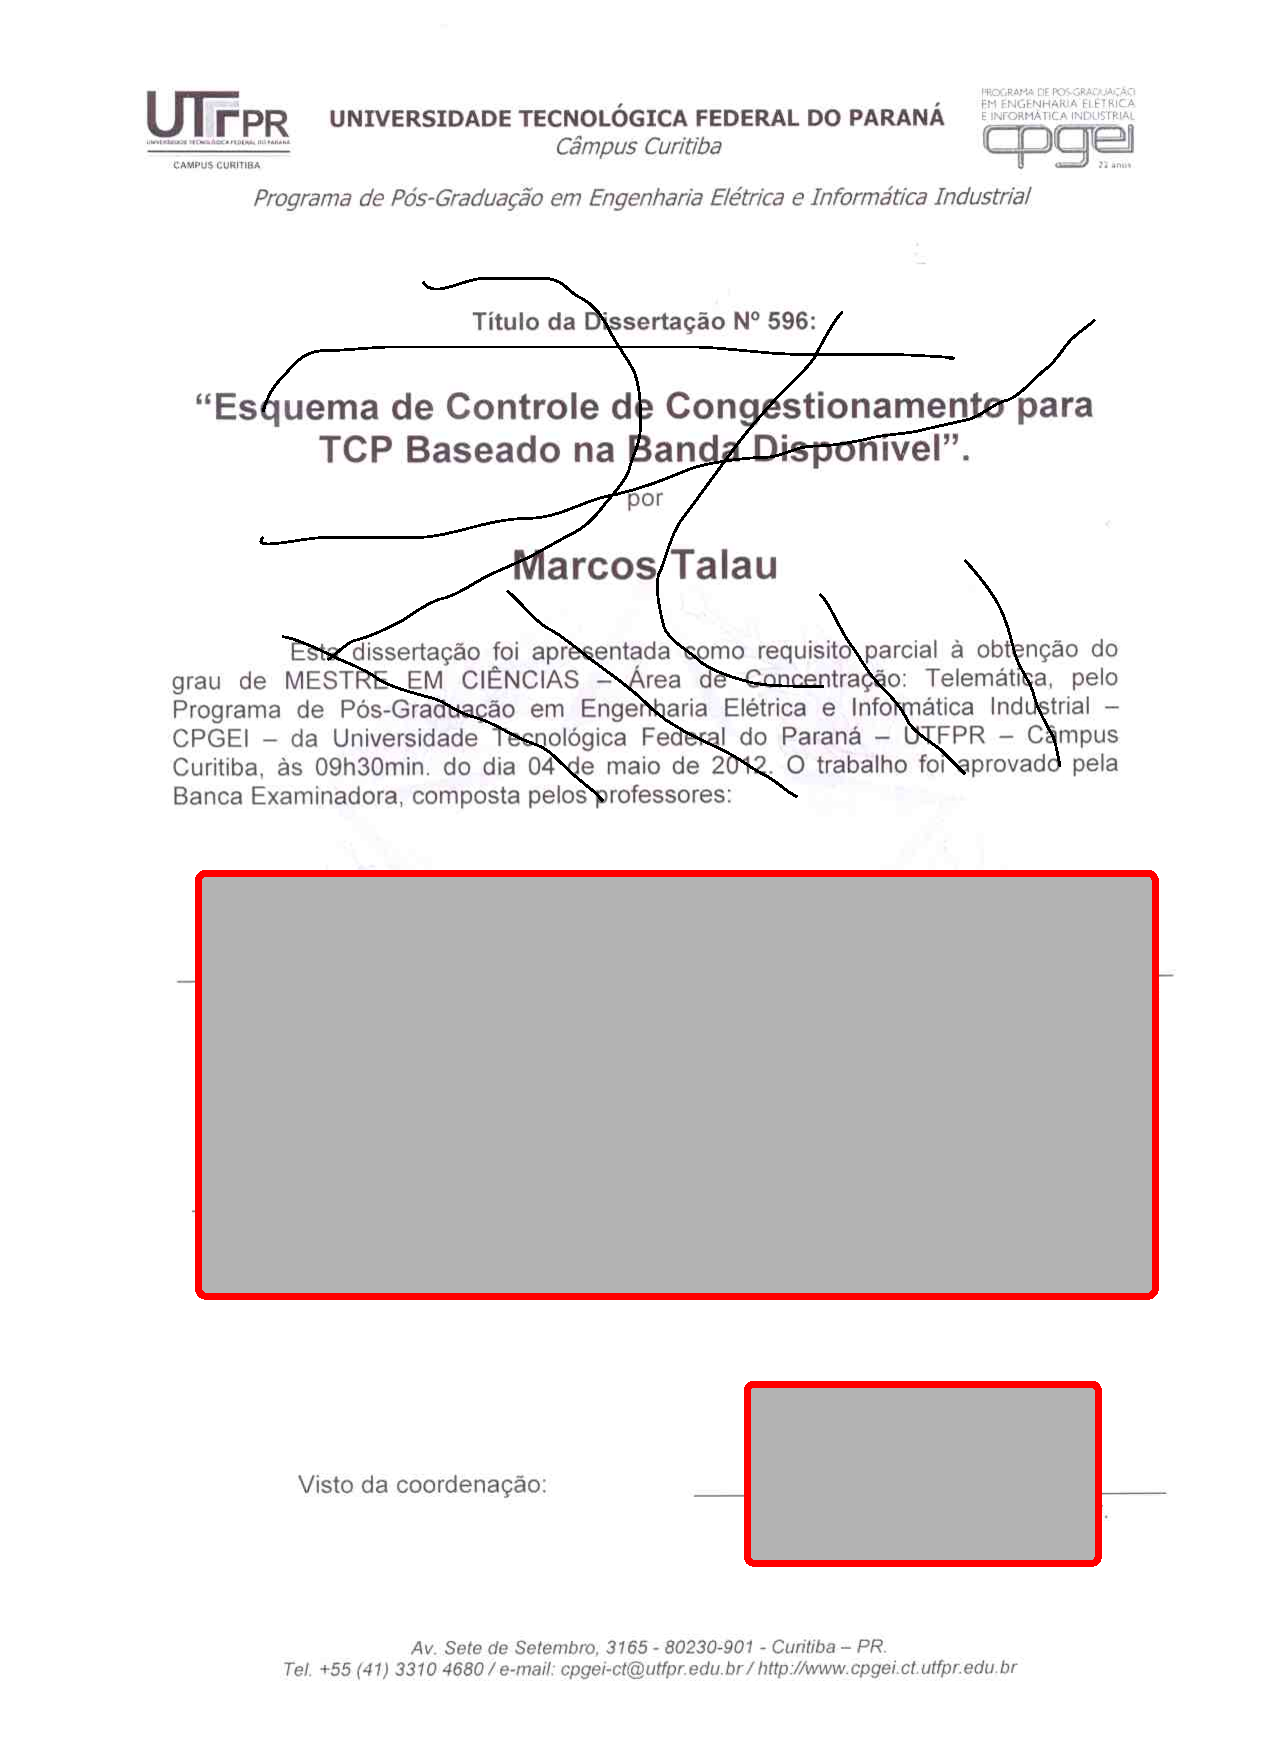
\includepdf{ata.pdf}

% dedicatoria
\begin{dedicatoria}
Texto da dedicat\'oria.
\end{dedicatoria}

% agradecimentos (opcional)
\begin{agradecimentos}
Texto dos agradecimentos.
\end{agradecimentos}

% epigrafe (opcional)
\begin{epigrafe}
Texto da ep\'igrafe.
\end{epigrafe}

%resumo
\begin{resumo}
Texto do resumo (m\'aximo de 500 palavras).
\end{resumo}

%abstract
\begin{abstract}
Abstract text (maximum of 500 words).
\end{abstract}

% listas (opcionais, mas recomenda-se a partir de 5 elementos)
\listadefiguras % geracao automatica da lista de figuras
\listadetabelas % geracao automatica da lista de tabelas
\listadequadros % adivinhe :)
\listadesiglas % geracao automatica da lista de siglas
\listadesimbolos % geracao automatica da lista de simbolos

% sumario
\sumario % geracao automatica do sumario


%---------- Inicio do Texto ----------
% recomenda-se a escrita de cada capitulo em um arquivo texto separado (exemplo: intro.tex, fund.tex, exper.tex, concl.tex, etc.) e a posterior inclusao dos mesmos no mestre do documento utilizando o comando \input{}, da seguinte forma:
%\input{intro.tex}
%\input{fund.tex}
%\input{exper.tex}
%\input{concl.tex}

\setcounter{page}{12}

%---------- Primeiro Capitulo ----------
\chapter{Introdução}

O presente documento \'e um exemplo de uso do estilo de formata\c{c}\~ao \LaTeX\ elaborado para atender \`as Normas para Elabora\c{c}\~ao de Trabalhos Acad\^emicos da UTFPR. O estilo de formata\c{c}\~ao {\ttfamily normas-utf-tex.cls} tem por base o pacote \textsc{abn}\TeX~-- cuja leitura da documenta\c{c}\~ao \cite{abnTeX2009} \'e fortemente sugerida~-- e o estilo de formata\c{c}\~ao \LaTeX\ da UFPR.

Para melhor entendimento do uso do estilo de formata\c{c}\~ao {\ttfamily normas-utf-tex.cls}, aconselha-se que o potencial usu\'ario analise os comandos existentes no arquivo \TeX\ ({\ttfamily modelo\_*.tex}) e os resultados obtidos no arquivo PDF ({\ttfamily modelo\_*.pdf}) depois do processamento pelo software \LaTeX\ + \textsc{Bib}\TeX~\cite{LaTeX2009,BibTeX2009}. Recomenda-se a consulta ao material de refer\^encia do software para a sua correta utiliza\c{c}\~ao~\cite{Lamport1986,Buerger1989,Kopka2003,Mittelbach2004}.

\begin{quadro}[!htb]
	\centering
	\caption[Exemplo de um quadro]{Exemplo de um quadro mostrando a correla\c{c}\~ao entre x e y.}
	\label{tab:correlacao}
	\begin{tabular}{cc}
		\hline 
		x & y \\
		\hline
		1 & 2 \\
		3 & 4 \\
		5 & 6 \\
		7 & 8 \\
		\hline 
	\end{tabular}
	\fonte{Autoria pr\'opria.}
\end{quadro}

\section{Motivação}

Uma das principais vantagens do uso do estilo de formata\c{c}\~ao {\ttfamily normas-utf-tex.cls} para \LaTeX\ \'e a formata\c{c}\~ao \textit{autom\'atica} dos elementos que comp\~oem um documento acad\^emico, tais como capa, folha de rosto, dedicat\'oria, agradecimentos, ep\'igrafe, resumo, abstract, listas de figuras, tabelas, siglas e s\'imbolos, sum\'ario, cap\'itulos, refer\^encias, etc. Outras grandes vantagens do uso do \LaTeX\ para formata\c{c}\~ao de documentos acad\^emicos dizem respeito \`a facilidade de gerenciamento de refer\^encias cruzadas e bibliogr\'aficas, al\'em da formata\c{c}\~ao~-- inclusive de equa\c{c}\~oes  matem\'aticas~-- correta e esteticamente perfeita.

\section{Objetivos}

\subsection{Objetivo Geral}

Prover um modelo de formata\c{c}\~ao \LaTeX\ que atenda \`as Normas para Elabora\c{c}\~ao de Trabalhos Acad\^emicos da UTFPR~\cite{UTFPR2008} e \`as Normas de Apresenta\c{c}\~ao de Trabalhos Acad\^emicos do DAELN~\cite{DAELN2006}.

\subsection{Objetivos Específicos}

\begin{itemize}
	\item Obter documentos acad\^emicos automaticamente formatados com corre\c{c}\~ao e perfei\c{c}\~ao est\'etica.
	\item Desonerar autores da tediosa tarefa de formatar documentos acad\^emicos, permitindo sua concentra\c{c}\~ao no conte\'udo do mesmo.
	\item Desonerar orientadores e examinadores da tediosa tarefa de conferir a formata\c{c}\~ao de documentos acad\^emicos, permitindo sua concentra\c{c}\~ao no conte\'udo do mesmo.
\end{itemize}


%---------- Segundo Capitulo ----------
\chapter{Desenvolvimento}
\label{chap:desenv}

A seguir ilustra-se a forma de incluir figuras, tabelas, equa\c{c}\~oes, siglas e s\'imbolos no documento, obtendo indexa\c{c}\~ao autom\'atica em suas respectivas listas. A numera\c{c}\~ao sequencial de figuras, tabelas e equa\c{c}\~oes ocorre de modo autom\'atico. Refer\^encias cruzadas s\~ao obtidas atrav\'es dos comandos {\ttfamily \textbackslash label\{\}} e {\ttfamily \textbackslash ref\{\}}. Por exemplo, n\~ao \'e necess\'ario saber que o n\'umero deste cap\'itulo \'e~\ref{chap:desenv} para colocar o seu n\'umero no texto. Isto facilita muito a inser\c{c}\~ao, remo\c{c}\~ao ou reloca\c{c}\~ao de elementos numerados no texto (fato corriqueiro na escrita e corre\c{c}\~ao de um documento acad\^emico) sem a necessidade de renumer\'a-los todos.

\section{Figuras}

Na figura~\ref{fig:dummy} \'e apresentado um exemplo de gr\'afico flutuante. Esta figura aparece automaticamente na lista de figuras. Para uso avan\c{c}ado de gr\'aficos no \LaTeX, recomenda-se a consulta de literatura especializada~\cite{Goossens2007}.


\begin{figure}[!htb]
	\centering
	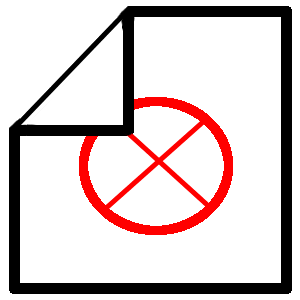
\includegraphics[width=0.2\textwidth]{./dummy.png} % <- formatos PNG, JPG e PDF
	\caption[Exemplo de uma figura]{Exemplo de uma figura onde aparece uma imagem sem nenhum significado especial.}
	\fonte{\cite{abnTeX2009}}
	\label{fig:dummy}
\end{figure}


\section{Tabelas}

Tamb\'em \'e apresentado o exemplo da tabela~\ref{tab:correlacao}, que aparece automaticamente na lista de tabelas. Informa\c{c}\~oes sobre a constru\c{c}\~ao de tabelas no \LaTeX\ podem ser encontradas na literatura especializada~\cite{Lamport1986,Buerger1989,Kopka2003,Mittelbach2004}.

\begin{table}[!htb]
	\centering
	\caption[Exemplo de uma tabela]{Exemplo de uma tabela mostrando a correla\c{c}\~ao entre x e y.}
	\label{tab:correlacao}
	\begin{tabular}{cc}
		\hline 
		x & y \\
		\hline
		1 & 2 \\
		3 & 4 \\
		5 & 6 \\
		7 & 8 \\
		\hline 
	\end{tabular}
	\fonte{Autoria pr\'opria.}
\end{table}

\section{Equações}

A transformada de Laplace \'e dada na equa\c{c}\~ao~(\ref{eq:laplace}), enquanto a equa\c{c}\~ao~(\ref{eq:dft}) apresenta a formula\c{c}\~ao da transformada discreta de Fourier bidimensional\footnote{Deve-se reparar na formata\c{c}\~ao esteticamente perfeita destas equa\c{c}\~oes!}.

\begin{equation}
X(s) = \int\limits_{t = -\infty}^{\infty} x(t) \, \text{e}^{-st} \, dt
\label{eq:laplace}
\end{equation}

\begin{equation}
F(u, v) = \sum_{m = 0}^{M - 1} \sum_{n = 0}^{N - 1} f(m, n) \exp \left[ -j 2 \pi \left( \frac{u m}{M} + \frac{v n}{N} \right) \right]
\label{eq:dft}
\end{equation}

\section{Siglas e símbolos}

O pacote \textsc{abn}\TeX\ permite ainda a defini\c{c}\~ao de siglas e s\'imbolos com indexa\c{c}\~ao autom\'atica atrav\'es dos comandos {\ttfamily \textbackslash sigla\{\}\{\}} e {\ttfamily \textbackslash simbolo\{\}\{\}}. Por exemplo, o significado das siglas\sigla{CPGEI}{Programa de P\'os-gradua\c{c}\~ao em Engenharia El\'etrica e Inform\'atica Industrial},\sigla{DAELN}{Departamento Acad\^emico de Eletr\^onica} e\sigla{UTFPR}{Universidade Tecnol\'ogica Federal do Paran\'a} aparecem automaticamente na lista de siglas, bem como o significado dos s\'imbolos\simbolo{$\lambda$}{comprimento de onda},\simbolo{$v$}{velocidade} e\simbolo{$f$}{frequ\^encia} aparecem automaticamente na lista de s\'imbolos. Mais detalhes sobre o uso destes e outros comandos do \textsc{abn}\TeX\ s\~ao encontrados na sua documenta\c{c}\~ao espec\'ifica~\cite{abnTeX2009}.


%---------- Terceiro Capitulo ----------
\chapter{Conclusão}

Espera-se que o uso do estilo de formata\c{c}\~ao \LaTeX\ adequado \`as Normas para Elabora\c{c}\~ao de Trabalhos Acad\^emicos da UTFPR ({\ttfamily normas-utf-tex.cls}) facilite a escrita de documentos no \^ambito desta institui\c{c}\~ao e aumente a produtividade de seus autores. Para usu\'arios iniciantes em \LaTeX, al\'em da bibliografia especializada j\'a citada, existe ainda uma s\'erie de recursos~\cite{CTAN2009} e fontes de informa\c{c}\~ao~\cite{TeX-Br2009,Wikibooks2009} dispon\'iveis na Internet.

Recomenda-se o editor de textos Kile como ferramenta de composi\c{c}\~ao de documentos em \LaTeX\ para usu\'arios Linux. Para usu\'arios Windows recomenda-se o editor \TeX nicCenter~\cite{TeXnicCenter2009}. O \LaTeX\ normalmente j\'a faz parte da maioria das distribui\c{c}\~oes Linux, mas no sistema operacional Windows \'e necess\'ario instalar o software \textsc{MiK}\TeX~\cite{MiKTeX2009}.

Al\'em disso, recomenda-se o uso de um gerenciador de refer\^encias como o JabRef~\cite{JabRef2009} ou Mendeley~\cite{Mendeley2009} para a cataloga\c{c}\~ao bibliogr\'afica em um arquivo \textsc{Bib}\TeX, de forma a facilitar cita\c{c}\~oes atrav\'es do comando {\ttfamily \textbackslash cite\{\}} e outros comandos correlatos do pacote \textsc{abn}\TeX. A lista de refer\^encias deste documento foi gerada automaticamente pelo software \LaTeX\ + \textsc{Bib}\TeX\ a partir do arquivo {\ttfamily reflatex.bib}, que por sua vez foi composto com o gerenciador de refer\^encias JabRef.

O estilo de formata\c{c}\~ao \LaTeX\ da UTFPR e este exemplo de utiliza\c{c}\~ao foram elaborados por Diogo Rosa Kuiaski (diogo.kuiaski@gmail.com) e Hugo Vieira Neto (hvieir@utfpr.edu.br), com contribui\c{c}\~oes de C\'esar Vargas Benitez. Sugest\~oes de melhorias s\~ao bem-vindas.


%---------- Referencias ----------
\clearpage % this is need for add +1 to pageref of bibstart used in 'ficha catalografica'.
\label{bibstart}
\bibliography{reflatex} % geracao automatica das referencias a partir do arquivo reflatex.bib
\label{bibend}

%---------- Apendices (opcionais) ----------
\apendice
\chapter{Nome do Ap\^endice}

Use o comando {\ttfamily \textbackslash apendice} e depois comandos {\ttfamily \textbackslash chapter\{\}}
para gerar t\'itulos de ap\^en-dices.


% ---------- Anexos (opcionais) ----------
\anexo
\chapter{Nome do Anexo}

Use o comando {\ttfamily \textbackslash anexo} e depois comandos {\ttfamily \textbackslash chapter\{\}}
para gerar t\'itulos de anexos.


% --------- Ordenacao Afabetica da Lista de siglas --------
%\textbf{* Observa\c{c}\~oes:} a ordenacao alfabetica da lista de siglas ainda nao eh realizada de forma automatica, porem
% eh possivel se de realizar isto manualmente. Duas formas:
%
% ** Primeira forma)
%    A ordenacao eh feita com o auxilio do comando 'sort', disponivel em qualquer
% sistema Linux e UNIX, e tambem em sistemas Windows se instalado o coreutils (http://gnuwin32.sourceforge.net/packages/coreutils.htm)
% comandos para compilar e ordenar, supondo que seu arquivo se chame 'dissertacao.tex':
%
%      $ latex dissertacao
%      $ bibtex dissertacao && latex dissertacao
%      $ latex dissertacao
%      $ sort dissertacao.lsg > dissertacao.lsg.tmp
%      $ mv dissertacao.lsg.tmp dissertacao.lsg
%      $ latex dissertacao
%      $ dvipdf dissertacao.dvi
%
%
% ** Segunda forma)
%\textbf{Sugest\~ao:} crie outro arquivo .tex para siglas e utilize o comando \sigla{sigla}{descri\c{c}\~ao}.
%Para incluir este arquivo no final do arquivo, utilize o comando \input{arquivo.tex}.
%Assim, Todas as siglas serao geradas na ultima pagina. Entao, devera excluir a ultima pagina da versao final do arquivo
% PDF do seu documento.


%-------- Citacoes ---------
% - Utilize o comando \citeonline{...} para citacoes com o seguinte formato: Autor et al. (2011).
% Este tipo de formato eh utilizado no comeco do paragrafo. P.ex.: \citeonline{autor2011}

% - Utilize o comando \cite{...} para citacoeses no meio ou final do paragrafo. P.ex.: \cite{autor2011}



%-------- Titulos com nomes cientificos (titulo, capitulos e secoes) ----------
% Regra para escrita de nomes cientificos:
% Os nomes devem ser escritos em italico, 
%a primeira letra do primeiro nome deve ser em maiusculo e o restante em minusculo (inclusive a primeira letra do segundo nome).
% VEJA os exemplos abaixo.
% 
% 1) voce nao quer que a secao fique com uppercase (caixa alta) automaticamente:
%\section[nouppercase]{\MakeUppercase{Estudo dos efeitos da radiacao ultravioleta C e TFD em celulas de} {\textit{Saccharomyces boulardii}}
%
% 2) por padrao os cases (maiusculas/minuscula) sao ajustados automaticamente, voce nao precisa usar makeuppercase e afins.
% \section{Introducao} % a introducao sera posta no texto como INTRODUCAO, automaticamente, como a norma indica.


\end{document}

